\documentclass[12pt,a4paper]{article}
\usepackage[margin=2.5cm]{geometry}
\usepackage{graphicx} % Required for inserting images
\usepackage{float}
\usepackage{subcaption}
\usepackage{booktabs}
\usepackage{parskip}
\usepackage{cleveref}


\title{A Comparison of Phase Recovery Algorithms for Energy Efficient Coherent Receivers}
\author{Joe Leacy}

\begin{document}

\maketitle

\section{Viterbi \& Viterbi}
Figure \ref{fig:viterbi_viterbi} shows the operation of the Viterbi-Viterbi algorithm. A block of symbols \(\left[z[k-N], z[k-N+1],\dots, z[k], \dots, z[k+N]\right]\) is raised to the
4th power to remove data dependency and convolved with a maximum-likelihood (ML) filter of length \(L = 2N + 1\) to compute \(\hat{\theta}_\mathrm{ML}[k]\).
A phase unwrapper is applied to reflect the unbounded Wiener phase noise, then the unwrapped phase correction is applied
to \(z[k]\). Here \(M = 4\) for QAM.
\begin{figure}[H]
    \centering
    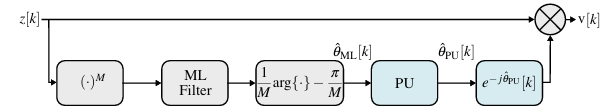
\includegraphics[width=0.8\textwidth]{viterbi_viterbi.png}
    \caption{Viterbi \& Viterbi algorithm block diagram}
    \label{fig:viterbi_viterbi}
\end{figure}
An energy efficient hardware implementation of this algorithm avoids multipliers where possible. The ML filter is known beforehand
so the multiplications can be replaced with fixed additions and shifts. Computing the argument of the filter output
and the phase correction can be implemented with CORDIC. The unwrapped phase is computed as
\[\hat{\theta}_\mathrm{PU}[k] = \hat{\theta}_\mathrm{ML}[k] + n[k]\frac{\pi}{2},\]
where \(n[k]\ \in \{-1, 0, 1\}\) is calcuated as  
\[n[k] = \left\lfloor\frac{1}{2} + \frac{\hat{\theta}_\mathrm{PU}[k-1] - \hat{\theta}_\mathrm{ML}[k]}{\pi/2}\right\rfloor.\]
The floor operation can be implemented efficiently with 2 comparators and division by \(\pi/2\) can be implemented as
multiplication by \(2/\pi\) with fixed shifts and additions as before. However the 4th power operation requires
complex multiplications which increase the energy cost. Assuming Gauss's algorithm for complex multiplication,
the total cost of this algorithm per symbol in terms of real multiplications (RM), real additions (RA), and bit-shifts
(BS) for \(n\)-bit fixed point precision with \(N_{C}\) CORDIC iterations is shown in Table \ref{tab:viterbi_viterbi_cost}. Note that the number
of shifts and adds for multiplication by a fixed value would be \(h\) and \(h-1\), where \(h\) is the Hamming weight, but here it is approximated as \(n\) for simplicity. The cost of a comparator operation is assumed to be the same as a real addition.
\begin{table}[H]
    \centering
    \begin{tabular}{lcccc}
        \toprule
        Operation & RM & RA & BS \\
        \midrule
        4th Power & \(9L\) & \(15L\) & 0 \\
        ML Filter & 0 & \(2(n-1)L\) & \(nL\) \\
        ML Phase & 0 & \(3N_C\) & \(2N_C\) \\
        Phase Unwrapper & 0 & \(5 + 2(n-1)\) & \(2n\) \\
        Phase Correction & 0 & \(3N_C\) & \(2N_C\) \\
        Total & 9L & \(2nL + 13L + 6N_C + 2n + 3\) & \(nL + 4N_C + 2n\) \\
        \bottomrule
    \end{tabular}
    \caption{Energy cost of Viterbi-Viterbi algorithm per symbol}
    \label{tab:viterbi_viterbi_cost}
\end{table}

\section{Blind Phase Search}
The Blind Phase Search algorithm is an alternative feed-forward algorithm that can be implemented without multipliers. Figure \ref{blind_phase_search} shows its operation. Producing the test rotations \(\theta_\mathrm{b}\) can be done very efficiently with CORDIC by reusing intermediate values, resulting in only \(\sum_{b=1}^{\log_2B} 2^{b+1} = 4B - 4\) shift and add operations for \(B\) rotations. For a QAM constellation \(\mathcal{S}\), the decision circuit is implemented with \(2(\sqrt{|\mathcal{S}|} - 1)\) comparators. Forming the squared distances \(|d_b[k]|^2\) appears to require a multiplier but the low degree of precision necessary means a look-up table (LUT) can be used. Additive noise is filtered from the estimate by summing \(L = 2N + 1\) squared distances. Finding the minimum \(m_b[k]\) can be done with \(B - 1\) comparators.
\begin{figure}[H]
    \centering
    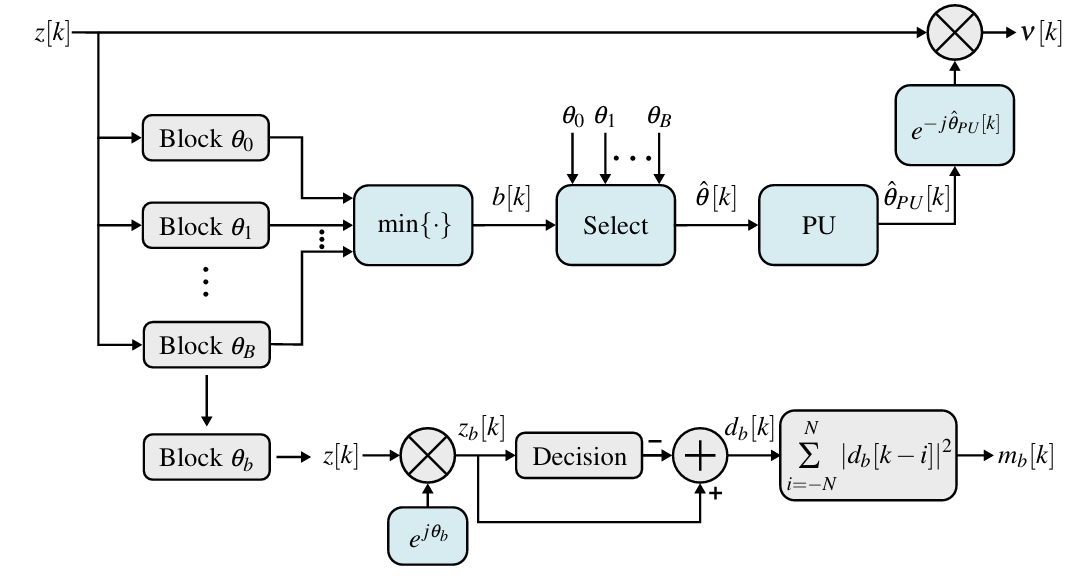
\includegraphics[width=0.8\textwidth]{blind_phase_search.png}
    \caption{Blind Phase Search algorithm block diagram}
    \label{blind_phase_search}
\end{figure}
The cost of this algorithm per symbol is shown in Table \ref{tab:blind_phase_search_cost}. For small constellations, the LUT will be small so accesses will be assumed to have negligible cost along with any MUX operations to select the correct \(\theta_\mathrm{b}\).
\begin{table}[H]
    \centering
    \begin{tabular}{lcccc}
        \toprule
        Operation & RM & RA & BS \\
        \midrule
        Test Rotations & 0 & \(4B - 4\) & \(4B-4\) \\
        Forming \(d_b[k]\) & 0 & \(2(\sqrt{|\mathcal{S}|} - 1) + 2\) & 0 \\
        Forming \(m_b[k]\) & 0 & L & 0 \\
        Minimum Search & 0 & \(B - 1\) & 0 \\
        Phase Unwrapper & 0 & \(5 + 2(n-1)\) & \(2n\) \\
        Phase Correction & 0 & \(3N_C\) & \(2N_C\) \\
        Total & 0 & \(5B + 2\sqrt{|\mathcal{S}|} + L + 2n + 3N_C - 2\) & \(4B + 2n + 2N_C - 4\) \\
        \bottomrule
    \end{tabular}
    \caption{Energy cost of Blind Phase Search algorithm per symbol}
    \label{tab:blind_phase_search_cost}
\end{table}

\section{Computational Cost}
As each stage of CORDIC applies a left bit-shift, the accuracy achieved by \(N_C\) iterations is approximately \(N_C\) bits.
Thus setting sensible values of \(N_C = n = 8\), \(L = 5\), \(|\mathcal{S}| = 16\), and \(B = 32\), the total cost of each algorithm is shown in Table \ref{tab:cost_comparison}.
\begin{table}[H]
    \centering
    \begin{tabular}{lcccc}
        \toprule
        Algorithm & RM & RA & BS \\
        \midrule
        Viterbi-Viterbi & 45 & 212 & 88 \\
        Decision-Directed & 0 & 71 & 92\\
        \bottomrule
    \end{tabular}
    \caption{Energy cost comparison of Viterbi \& Viterbi and Decision-Directed algorithms per symbol}
    \label{tab:cost_comparison}
\end{table}
It is clear the the Blind Phase Search algorith is more energy efficient. This is due to the absence of multipliers, a simpler additive noise filter, and efficient reuse of intermediate values for test rotations.
\section{Block-Wise Correction}
Both the Viterbi-Viterbi and Blind Phase Search algorithms can operate on blocks of symbols to reduce their computational cost. An estimated phase can be found for one symbol in a block of \(K\) and applied to the whole block, thereby reducing the cost by a factor of \(K\). However, this reduces the accuracy of the phase estimate and can make cycle slips more likely in the phase unwrapper. Pilot symbols can be used in both algorithms to mitigate this issue. (plot of BER vs block size for both algorithms with and without pilots using values above).
\section{Simplified Blind Phase Search}
Try removing additive noise filter.


\end{document}